Macros
\newcommand{\mctp}{\ensuremath{M_{\mathrm{CT}\perp}}}

Abstract:Change sentence the sentence (Final states with three leptons…) to read

Final states with three leptons, with a same-sign lepton pair, and with an opposite-sign lepton pair inclusive and in conjunction with two jets, are examined.

Introduction:

Line 11: In this paper, we present dedicated searches for chargino-neutralino and chargino pair production.

(Do we want to put something about the slepton model in here? This would require re-writing everywhere EWKino->weakly-produced SUSY)

Line 41: We also present results for a closely related model with the same decays, but chargino-chargino production instead of chargino-neutralino production, yielding a two lepton final state. This is depicted in \ref{fig:TChipmSlepSnuDiagram.pdf}. Note that in each event, each chargino can decay via either of the modes shown in the figure. Thus, there are 4 different decay pairs, but all 4 give similar dilepton plus \MET final states.

Finally, we present results of an non-resonant opposite-sign dilepton search in terms of direct slepton pair production, with each slepton decaying a lepton and a neutralino. This scenario is shown in Fig. \ref{fig:TSlepSlepDiagram.pdf}

Line 83 (Section 5…) Section 5 describes two dilepton searches, one for the on-shell W and Z boson production processes of Fig. 2 and another for off-Z dilepton events produced by chargino pair production with decays as in Fig. 1.

Section 5:

Make two subsections, one for my analysis, and one for Ben's.

My subsection: Searches in non-resonant opposite sign dileptons plus \MET.

This search looks for events with two opposite sign leptons that are not consistent with a Z boson and \MET. Here, the word lepton indicates an electron or muon. Both leptons are required to have $\pt > 20 \GeV$ and we require $\MET > 60 \GeV$, and the dilepton invariant mass at least 15 \GeV away from the Z peak at 91 GeV. This leaves mostly SM backgrounds where both leptons and \MET come from leptonic W decays, primarily dileptonic \ttbar decays and direct WW production. We eliminate some of the \ttbar background by vetoing jets that are tagged as coming from b quarks.

The remaining \ttbar and WW background can be greatly reduced by a cut on the \mctp\ variable, described in \cite{Matchev:2009ad}. This variable is expected to have a kinematic limit at the W boson mass of 80.4 \GeV when both leptons and \MET originate from W bosons. Since imperfect kinematic measurements can lead to events slightly beyond this limit, we require $\mctp > 100 \GeV$.

The Standard Model background is estimated using templates describing the \mctp\ shapes for the different background types. First, an \mctp\ histogram is derived for each background type from either a control sample or Monte Carlo simulation. Then, the low \mctp\ ($5 < \mctp < 100 \GeV$) region of the data is fit to a sum of these templates, when the number of events contributed by each background template determined by the fit. This provides an estimate of the overall normalization for each template. Finally, the normalizations are combined with the complete templates to predict the number of events in the signal region from each background type.

The template shape for backgrounds containing top quarks is estimated from a control sample of events containing one or more identified b jets. For this background, it is straightforward to estimate the number of events passing the b jet veto using an average b tagging efficiency determined from the ratio of the number of events with two identified b jets to the number with one. This information is added to the template fit as a Gaussian constraint.

The template for events with one real lepton and one fake lepton (originating mostly from W boson plus jet production) is determined from data using a control region of events with one isolated lepton and one lepton in a less-isolated sideband. A single template is used for diboson events, including WW, WZ, and ZZ production. This template comes from Monte Carlo simulation. Similarly, a template for backgrounds with two leptons from an off-shell Z plus fake \MET is obtained from simulation. Comparison of data and Monte Carlo simulation in the Z peak confirms that this background is well-modelled by the simulation. \fixme{Is there room for this plot here?}

Figure \ref{fig:OSDil_MCTDistribution} shows the \mctp\ distribution in data overlaid on the Monte Carlo simulation. Table \ref{tab:osdilresults} shows background predictions, along with data yields in the signal region. \fixme{Conclusions go here}

fig:OSDil_MCTDistribion
tab:osdilresults


Section 6: Add two subsections, one for TChipmSlepSnu, one for TSlepSlep.

Figure \ref{fig:MCTLimits} shows limits on chargino pair production cross section times branching ratio for charginos decaying as in Fig. \ref{fig:TChipmSlepSnuDiagram} (left) and for slepton pair production with decays as in Fig. \ref{fig:TSlepSlepDiagram}. These limits are set by the \mctp\ based analysis, and are for the flavor-democratic scenario with $x_{\PSlep}=0.5$. The contours show the 95\% exclusion contour given the MSSM cross-section.

Summary: This will need some mention of the mct analysis

## Figures:

\begin{figure}
    \begin{center}
        \fixme{Waiting on Wolfgang for this diagram}
        % \includegraphics[]{fig:TChipmSlepSnuDiagram}
        \caption{Diagrams for chargino pair production in proton-proton collisions and subsequent decay via sleptons and sneutrinos, leading to final states with two leptons, two LSPs, and two neutrinos. Note that either chargino can decay via either mode, giving 4 possible diagrams. However, all diagrams share the same final state.}
        \label{fig:TChipmSlepSnuDiagram}
    \end{center}
\end{figure}

\begin{figure}
    \begin{center}
        \fixme{Waiting on Wolfgang for this diagram}
        % \includegraphics[]{fig:TSlepSlepDiagram}
        \caption{Diagrams for slepton pair production in proton-proton collisions and decay to leptons and LSPs, leading to final states with two leptons and two LSPs. Sleptons produced belong to the same lepton flavor, so the final state leptons also share the same flavor.}
        \label{fig:TSlepSlepDiagram}
    \end{center}
\end{figure}

\begin{figure}
    \begin{center}
        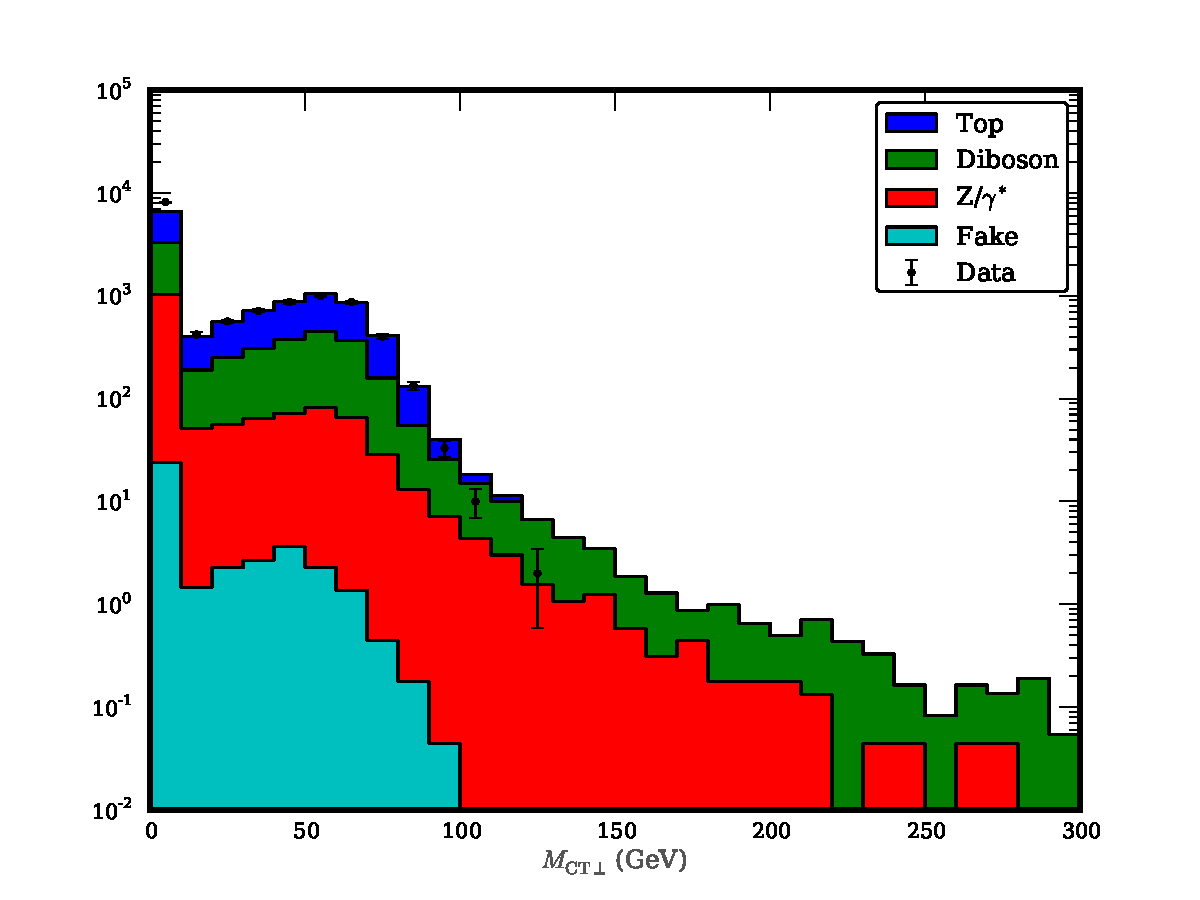
\includegraphics[]{OSDil_MCTDistribution}
        \caption{The \mctp\ distribution in data (black points) and expectations from Monte Carlo simulation (filled histogram). Notice that the Standard Model backgrounds in the simulation fall off dramatically above about 80 \GeV. The number of events in the $\mctp > 100\GeV$ signal region is consistent with the prediction of a partially data-driven background estimate.}
        \label{fig:OSDil_MCTDistribution}
    \end{center}
\end{figure}

## Table:
OSDil_ResultsTable.tex

## Bib:
@article{Matchev:2009ad,
      author         = "Matchev, Konstantin T. and Park, Myeonghun",
      title          = "{A General method for determining the masses of
                        semi-invisibly decaying particles at hadron colliders}",
      journal        = "Phys.Rev.Lett.",
      volume         = "107",
      pages          = "061801",
      doi            = "10.1103/PhysRevLett.107.061801",
      year           = "2011",
      eprint         = "0910.1584",
      archivePrefix  = "arXiv",
      primaryClass   = "hep-ph",
      SLACcitation   = "%%CITATION = ARXIV:0910.1584;%%",
}
